\section{Localisation}
\label{sec:localisation}

Now that we can extract a matching score from the paintings, we can use this to deduce the room we're currently in. If we only use the matching score our room prediction would be very heavily influenced by possible mismatches. This is why we opted for the use of a hidden Markov model (HMM).

\subsection{Hidden Markov Model}
A hidden Markov model is a statistical model that can combine the matching score with spatio-temporal features to become a room prediction. This is perfect for our assignment because, as stated previously, a prediction that's only based on the matching score would be very dependent on the quality of the matching algorithm which would make it very susceptible to mismatches.

\subsubsection{Architecture}
The underlying architecture of a HMM consists of 2 layers, a hidden layer and a layer with observed variables. The hidden layer consists of the transition probabilities between different states. The observed variables are observations that belong to a certain state with a certain probability. In this project, these "states" represent the different rooms, while the transition probability stands for the probability that a person stays in the current room or goes from the current room to another room. The processed video frames are the observed variables, where the probability of this frame belonging to a certain state/room is calculated by using the matching score of multiple matches. An example of the hidden Markov model architecture is shown in figure \ref{fig:hmm}.


\begin{figure}[htbp]
    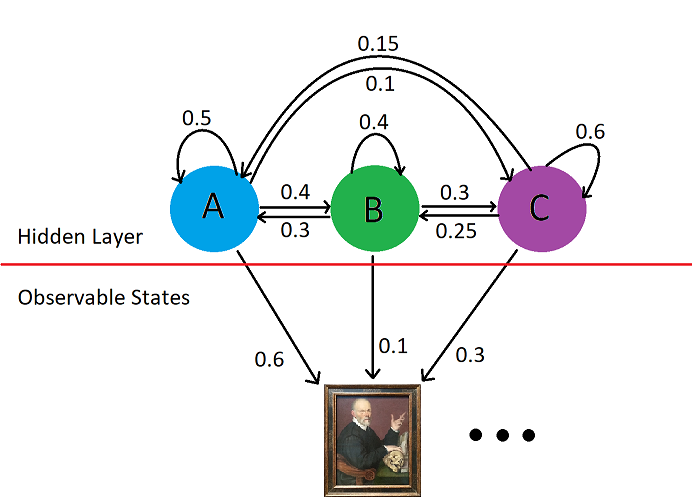
\includegraphics[width=\linewidth]{images/hmm.png}
    \caption{Hidden Markov Model architecture}
    \label{fig:hmm}
\end{figure}

\subsubsection{Calculating the transition probabilities}
The amount of rooms between the start and destination room is used as a metric to calculate the transition probabilities between the rooms. If there are more rooms between the two rooms, the probability of the next frame being in the destination room would be lower than when the start and destination room would be adjacent. The reasoning behind this is pretty straightforward. It’s simply very unlikely that a person goes from a certain room to the other side of the museum in a matter of seconds.
To apply this in our program, we first need to know the number of rooms that are between the start and destination room. Note that we only have the floor plan of the museum to start with. Starting from this floor plan, an undirected graph was created where the connected nodes represent the adjacent rooms. After creating this graph, we extract the adjacency matrix to become a matrix structure that shows the adjacent rooms.
From this adjacency matrix, we can calculate the distance matrix by using the Floyd Warshall algorithm \cite{floyd_warshall}, which is an algorithm that’s used to calculate the optimal path between all the different nodes in a graph.
Now that the distance matrix is calculated, a distribution has to be applied to the rows which makes sure that the shortest distances have the highest probability, while the longest distances have the lowest probability. For this project, a linear and a Gaussian distribution were created and after extensive testing, the Gaussian distribution with $\mu = 0$ and $\sigma = 1$ was found to be the best performing distribution. \par 
The process to create the transition probabilities is visualized below for the example in fig. \ref{fig:hmm} where we assume that the rooms are in a straight line (A - B - C). We start from the connectivity matrix, to become the distance matrix and end up with the probability matrix after applying the Gaussian distribution.

\[
\begin{bNiceMatrix}[first-row,first-col]
  & A & B & C \\
A & 0 & 1 & 0 \\
B & 1 & 0 & 1 \\
C & 0 & 1 & 0 
\end{bNiceMatrix} 
\Rightarrow
\begin{bmatrix}
0 & 1 & 2 \\
1 & 0 & 1 \\
2 & 1 & 0 \\
\end{bmatrix}
\Rightarrow
\begin{bmatrix}
0,58 & 0.35 & 0.07 \\
0.27 & 0.46 & 0.27 \\
0.07 & 0.35 & 0.58 \\
\end{bmatrix}
\]

%\begin{figure}[htbp]
%    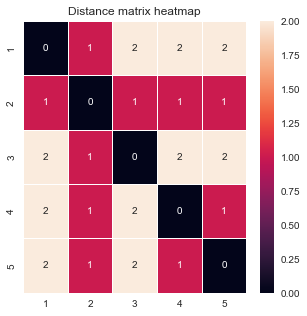
\includegraphics[width=\linewidth]{images/distance_matrix_5x5.png}
%    \caption{Distance Matrix HMM (5x5)}
%    \label{fig:distance_matrix_5x5}
%\end{figure}

\subsubsection{Calculating the probabilities for the observable variables}
Next up,  the probabilities for the observable variables have to be calculated. The observable variables in the HMM are the frames that are effectively processed and matched against the database. The probabilities are calculated based on the matching scores (distance with ORB) from the extracted contours.
The algorithm goes as follows:
For every extracted contour, the best matching score (lowest = best) is taken for each possible room based on the list of soft matches from that contour. The room scores for every room are then added together. Based on this list of scores for every room, the probability is calculated so the lowest score gets the highest probability and similar scores get similar probabilities. To reduce the effect of mismatches, the probability of the previous room is set to 2\% if there are no soft matches for that room.
\\
\subsubsection{Making the room prediction}
To make the room prediction, the transition probabilities are combined with the probabilities for the observable variables.
For every room, the probability is calculated by using the forward algorithm \cite{blunsom2004hidden} \cite{ahmadian2018systematic}, which is a dynamic algorithm that uses the following formula to calculate the probability of the frame being in a certain room $\alpha_t(x_t)$.  \[ \alpha_t(x_t) = p(y_t|x_t) \sum_{x_{t-1}}p(x_t|x_{t-1})\alpha_{t-1}(x_{t-1}) \] 
This formula simply calculates the chance that the current frame is in a certain room, based on the probabilities for each room in the previous frame $p(x_t|x_{t-1})\alpha_{t-1}(x_{t-1})$. The room probabilities based on the matching score alone are represented as $p(y_t|x_t)$. When processing the first frame no previous prediction exists. Therefore, the stationary distribution $\pi$ is used for the first frame. The stationary distribution represents the row vector such that $\pi = \pi P$, where $P$ represents the hidden layers of the model. By using this, we become starting probabilities where the rooms with more neighbors get a higher probability.\par

After applying the forward algorithm, the location prediction is obtained by simply selecting the room with the highest probability.


\subsection{Hidden Markov Model visualization}

The room predictions from the hidden Markov model are extracted and used to color-code a floor plan of MSK Ghent (see figure \ref{fig:hmm-viz}). Every room is assigned to a color between red and green where the colors correspond to a low, respectively high percentage of currently being in that room. The top three predictions of the most likely rooms are also displayed in the bottom-left part of the image with the prediction percentage. 
The rooms with the highest percentages in time are also connected with lines to show the traveled path on the floor plan of MSK Ghent.

\begin{figure}[htbp]
    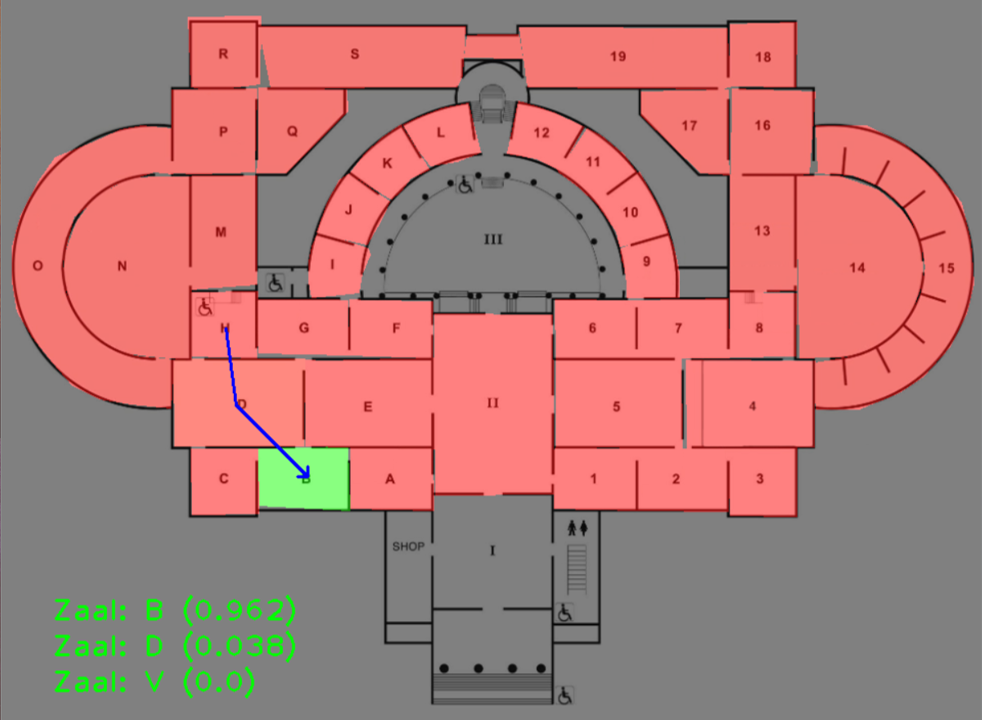
\includegraphics[width=\linewidth]{images/hmm-vis.png}
    \caption{Hidden Markov Model visualization}
    \label{fig:hmm-viz}
\end{figure}